\section{Ejercicio 3}

% El nuevo problema que tienen Marty y el Doc es que ahora no se ponen de
% acuerdo en qué estructura quı́mica deben utilizar para armar el condensador
% de flujos. Marty, a partir de las propiedades atómicas, ha obtenido una
% constante n y está seguro de que la solución que están buscando debe ser un
% grafo de a lo sumo n vértices (o como él lo dice, un subgrafo de algún Kn),
% mientras que el Doc ha estudiado las caracterı́sticas moleculares e insiste
% con que debe ser un subgrafo de un cografo dado. Por las dudas, y para
% evitar más conflictos entre ellos, quieren cumplir con ambas
% especificaciones, siempre maximizando la cantidad de aristas, dado que éste
% es el punto clave para su funcionamiento dentro del condensador. Por eso les
% pedimos que los ayuden diseñando e implementando un algoritmo exacto para
% MCS que tenga complejidad temporal polinomial para el caso en el que G1 es
% un cografo y G2 es un grafo completo y desarrollen los siguientes puntos que
% avalen la solución encontrada (si estamos hablando de viajar en el tiempo,
% no hay margen de error posible):
% a) Explicar detalladamente el algoritmo implementado.
% b) Calcular el orden de complejidad temporal de peor caso del algoritmo.
% c) Realizar una experimentación que permita observar los tiempos de
%    ejecución del algoritmo en función del tamaño de entrada.

\subsection{Introducción}
En este ejercicio, se busca encontrar un algoritmo exacto para resolver, en
tiempo polinomial, el problema del \acr{MCS} entre dos grafos cuando uno de
ellos es un grafo completo y el otro es un \emph{cografo}. La clase de los
cografos, o grafos reducibles por complemento, se define recursivamente y
consiste exactamente en los grafos que pueden construirse según alguna de las
siguientes reglas:
\begin{enumerate}
    \item Un nodo aislado ($K_1$) es un cografo.
    \item La unión de dos o más cografos es un cografo.
    \item El complemento de un cografo es un cografo.
\end{enumerate}

Es posible demostrar (\cite{corneil}, Corneil et al.) que todo cografo
admite una representación mediante un árbol enraizado, que se conoce como
coárbol (o \emph{cotree}) del mismo. Existen diferentes variantes de esta
representación, pero en todas ellas las hojas del árbol corresponden a los
nodos del grafo, mientras que los nodos internos representan el cografo que se
obtiene aplicando una determinada operación a los cografos relativos a sus
nodos hijos. Así, la raíz del coárbol se corresponde con el cografo completo
que se busca representar.

% Para obtener esta representación se parte de que todo cografo, o bien es una
% unión disjunta de cografos, o su complemento lo es. De esto se sigue que
% todo cografo puede reducirse a un conjunto de nodos aislados complementando
% de forma sucesiva sus componentes conexas (de allí que a estos grafos se los
% conozca como \emph{reducibles por complemento}). Esto equivale a decir que
% puede darse una forma iterativa para construir cualquier cografo a partir de
% sus nodos; se comienza considerando todos ellos como grafos disjuntos, y
% luego se conectan estos grafos iterativamente computando en cada paso el
% complemento de la unión de algunos de ellos. Dado un cografo cualquiera, su
% coárbol no es más que la representación de este proceso mediante un árbol:
% las hojas del mismo corresponden a los nodos del cografo, y cada nodo
% interno representa el complemento de la unión de los cografos
% correspondientes a sus hijos. El cografo en sí mismo es representado la raíz
% del árbol.

En este trabajo, las dos operaciones que se utilizarán para etiquetar los
nodos internos de un coárbol provienen de una definición alternativa y
equivalente de cografo: un grafo es un cografo si y solo si puede obtenerse a
partir de nodos aislados mediante la aplicación sucesiva de la unión disjunta
($\cup$) y el \emph{join} ($\times$). Esta última operación se define de la
siguiente forma: dados $G_1, \dots, G_k$ grafos, el \emph{join} entre ellos es
el grafo $G_1 \times \dots \times G_k = \left((G_1)\comp \cup
\dots \cup (G_k)\comp\right)\comp$. Una forma más intuitiva de pensar el
\emph{join} entre grafos es partir de la unión disjunta entre ellos, y agregar
todas las aristas cuyos extremos se encontraban en grafos distintos.

Otra consideración a tener en cuenta es que, para simplificar la
implementación, se utilizarán coárboles estrictamente binarios; es decir,
cada nodo interno representará una operación entre exactamente dos cografos.
Esto no resulta problemático, ya que tanto la unión como el \emph{join} entre
grafos son operaciones asociativas.

\begin{figure}[htbp]
    \centering
    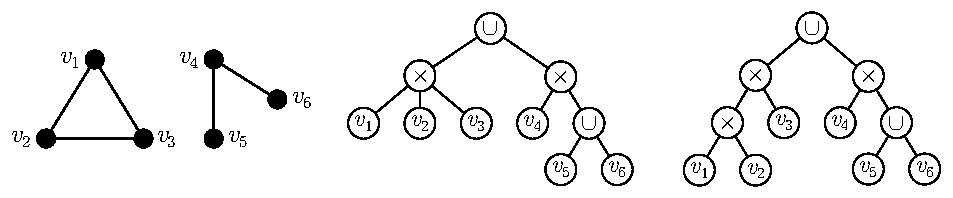
\includegraphics{imagenes/cografos-ejemplo-coarbol.pdf}
    \caption{Ejemplo de un cografo, su coárbol correspondiente, y la
    representación estrictamente binaria del mismo.}
    \label{fig:cografos:ejemplo-coarbol}
\end{figure}

\subsection{Resolución algorítmica}


\subsection{Detalles implementativos}

\subsection{Complejidad}

\subsection{Experimentación}
